%!TEX root = ../Fast_Contour_Tracing_Algorithm.tex
% -*- root: ../Fast_Contour_Tracing_Algorithm.tex -*-

\section{Proposed Contour Tracing Algorithm}

In this section, we propose a novel pixel following algorithm that traces contour pixels by considering their local patterns. Therefore, it can classify the contour pixel into contour types such as inner corner, outer corner, inner-outer corner, and straight line; further, it can easily determine the next contour pixel. Moreover, it can determine and save representative points of an image, like the RD code method, by using pixel following but not using run-data-based following. In addition, the data can be restored to the original contour pixels without the RD code data.

\subsection{Contour Following}

\subsubsection{Assumptions for start-up and stopping criteria}
The proposed algorithm runs under two assumptions for start. One is the general condition for pixel following: the rear pixel of the tracer on the start pixel is white. The other is that there is no left-rear inner-outer corner for the tracer at the start position, i.e., if the rear and the left pixels are white and the rear-left pixel is black, the start pixel has to be changed. These are the same starting conditions as those for the MSBF and ISBF. Moreover, the stop criteria of the proposed algorithm is Jacob's stopping criterion and the tracer is always on a contour pixel.

\begin{figure}[htbp]
	\centering
	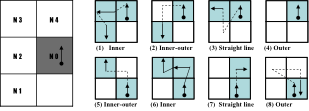
\includegraphics[width=1.0\textwidth]{4.Proposed/proposed_cases.png}
	\caption{Contour tracing cases of the proposed contour following algorithm.}
	\label{fig:proposed_cases}
\end{figure}


\subsubsection{Procedures}

The proposed algorithm has two stages. First, the tracer follows the contour pixel on the basis of the intensities of the left-rear and left pixels. After that, the tracer follows the contour pixels on the basis of the intensities of the front and front-left pixels. Figure \ref{fig:proposed_cases} shows the contour tracing cases of the proposed contour following algorithm. In the figure, the tracer is first on N0 queries states of $N1$ and $N2$, as shown in figure \ref{fig:proposed_cases} (a), and then the states determine the corresponding  path to trace among cases (1)-(4), as shown in figure \ref{fig:proposed_cases} (b). After stage 1, the moved tracer queries states N3 and N4 and then it traces contour pixels along the corresponding path using the states among cases (5)-(8). 

Hence, by using the proposed algorithm, the inner corners are traced as case (1) or case (6), the inner-outer corners are traced as case (2) or case (5), the outer corners are determined as case (4) or case (8), and the straight-line pixels are determined as the other cases. Therefore, all the cases are easily classified by using the algorithm. 




\subsubsection{States}

\begin{figure}[htbp]
	\centering
	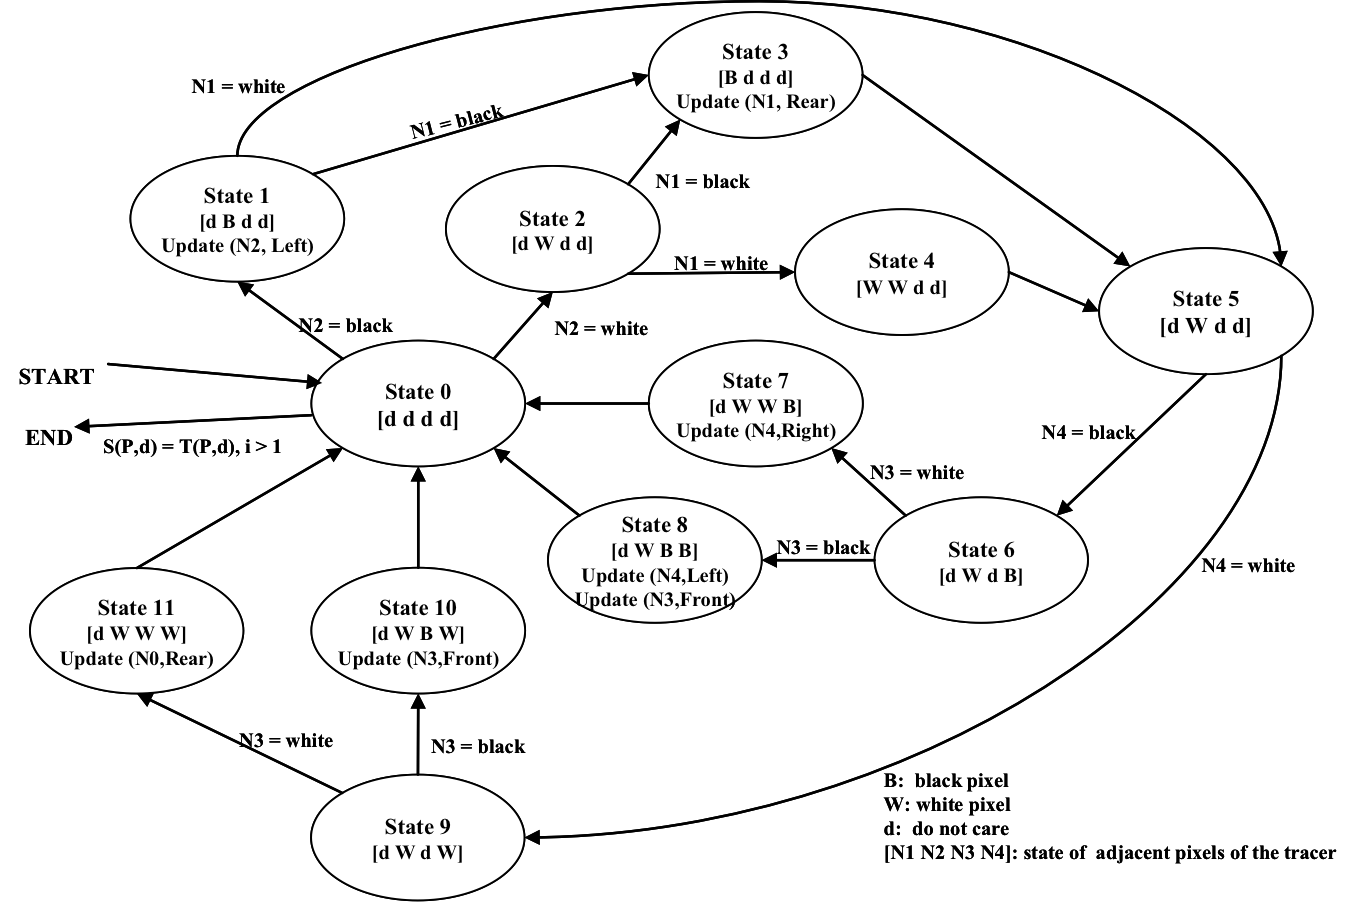
\includegraphics[width=1.0\textwidth]{4.Proposed/state.png}
	\caption{The state transition of the automation for the proposed algorithm.}
	\label{fig:state}
\end{figure}

Figure \ref{fig:state} describes the state transition for the automation of the proposed algorithm. In the figure, the start and termination occur at State 0; the first stage runs using States 1-4 and then it transits to State 5. The second stage continues from State 5 using States 6-11 and then it transits to State 0. For example, case (1) in figure \ref{fig:proposed_cases} can be executed by the transit sequence State 1, State 3, and State 5. 

In figure \ref{fig:state}, $[N1 N2 N3 N4]$ represents the intensity vector of the tracer's four adjacent pixels shown in figure \ref{fig:proposed_cases} (a). In the vector, $d$ implies ``do not care''; $B$, a contour pixel (black); and $W$, the background pixel (white). Moreover, Update $(P,d)$ refers to the movement operation where P is the new contour pixel location and $d$ is the new directional information for the tracer. In State 1 and State 3, the updates occur based on the tracer of State 0, and other updates are based on the tracer information in State 5.

\subsubsection{Characteristics of the proposed algorithm}

We designed the proposed algorithm based on two stages with two major goals. First, the check operation for stopping occurs only at State 0; therefore, the number of checking operations on black pixels are reduced. In other words, the proposed algorithm examines that the check operation occurs when only the tracer has a white rear pixel. This is more efficient as compared to the check operation occuring for every contour pixel because its start condition and stop criterion also satisfy that the rear pixel of the tracer on the start pixel is white. Therefore, the transition of stage 2 to States 6 to 11 for processing cases (5) to (8) is designed such that it can be returned to State 0 only if the tracer has a white rear pixel, and it reduces any unnecessary operations for checking to stop. Besides, the tracers of cases (2) and (4) have a white rear pixel after movement but their end conditions are not considered. In case (2), at the start the tracer avoids the inner-outer corner pixels as the start and end pixel. Moreover, in case (4), the tracer has no update; therefore, it is unnecessary to perform check operation twice. 

Second, the proposed algorithm reduces some of the redundant operations used for detecting white pixels. The conventional algorithms do not consider white pixels in the previous path; therefore, they sometimes redetect white pixels on the previous tracing during the current tracing. For example, in figure 8, the white pixel at (4, 2) is detected twice while determining contour pixels such as (4, 3) and (5, 3). Moreover, RSA detects (4, 2) three time while determining (4, 3), (5, 3), and (6, 3). On the contrary, the proposed algorithm has two stages and its second stage avoids the previous path. \textcolor{red}{Figure 11} shows the contour tracing results for the proposed algorithm and it detects (4, 2) once for contour tracing. Moreover, the figure shows that the proposed algorithm has fewer operations on the white pixels as compared to conventional pixel following methods, as shown in figure \ref{fig:comparison}, and traces all the types of contours. 

The pseudo-code of the proposed algorithm is as below: 

\begin{algorithm}
\caption{Algorithm of Proposed Algorithm}
\label{alg:proposed}
\begin{algorithmic}[1]
\Procedure{Proposed\_Tracer}{}
\State $\textit{T(P,d)} \gets \textit{S(P,d)}$, where $P$ is on black, $P_{Rear}$ is on white and $i \gets 1$
\LineComment{Whenever $T(P,d)$ is updated, $i$ increases $1$ and $T(p',d')$ is saved automatically}
\Do
\LineComment{State 1}
\If {$\textit{P}_{Left-Rear}$ = black}
	\If {$\textit{P}_{Left}$ = black}
		\LineComment{Case 1}
		\State $\textit{T(P,d)} \gets \textit{T(P}_{Left},\textit{d}_{Left} )  $ and $\textit{Code(i)} \gets ``Inner''$ and $\textit{T(P,d)} \gets \textit{T(P}_{Left}, \textit{d}_{Left})$
	\Else
		\LineComment{Case 2}
		\State $\textit{Code(i)} \gets ``Inner-outer''$ and $\textit{T(P,d)} \gets \textit{T(P}_{Left-Rear},\textit{d}_{Rear} )  $
		\State $\textit{Code(i)} \gets ``Inner-outer''$
	\EndIf
\Else
	\If {$\textit{P}_{Left}$ = black}
		\LineComment{Case 3}
		\State $\textit{T(P,d)} \gets \textit{T(P}_{Left},\textit{d}_{Left} )  $ and $\textit{Code(i)} \gets ``Straight''$
	\Else
		\LineComment{Case 4}
		\State $\textit{Code(i)} \gets ``Outer''$
	\EndIf
\EndIf


\LineComment{Stage 2}
\If {$\textit{P}_{Front-Left}$ = black}
	\If {$\textit{P}_{Front}$ = black}
		\LineComment{Case 6}
		\State $\textit{T(P,d)} \gets \textit{T(P}_{Front},\textit{d}_{Left} )  $ and $\textit{Code(i)} \gets ``Inner''$ and $\textit{T(P,d)} \gets \textit{T(P}_{Front}, \textit{d}_{Right})$
	\Else
		\LineComment{Case 5}
		\State $\textit{Code(i)} \gets ``Inner-outer''$ and $\textit{T(P,d)} \gets \textit{T(P}_{Front-Left},\textit{d} )  $
		\State $\textit{Code(i)} \gets ``Inner-outer''$
	\EndIf
\ElsIf {$\textit{P}_{Front}$ = black}
	\LineComment{Case 7}
	\State $\textit{T(P,d)} \gets \textit{T(P}_{Front},\textit{d}_{Right} )  $
\Else
	\LineComment{Case 8}
	\State $\textit{T(P,d)} \gets \textit{T(P},\textit{d}_{Rear} )  $ and $i \gets i-1$ and $\textit{Code(i)} \gets ``Outer''$
\EndIf


\doWhile {$ \textit{T(P,d)}  \neq \textit{S(P,d)}$}
\EndProcedure
\end{algorithmic}
\end{algorithm}

Table \ref{table:proposed_result} describes the tracing results obtained by using the proposed algorithm up to the stage the tracer enters the 11th pixel. The code represents the contour pixel type and it is classified automatically during tracing. 

\begin{table}[h]
	\centering
	% \begin{tabularx}{0.7\textwidth}{*{4}{Y}}
	\begin{tabularx}{0.7\textwidth}{Y|Y|Y|Y}
\hline
\hline
\multirow{2}{*}{$Sequence(i)$} &  \multicolumn{2}{|c|}{P}  & \multirow{2}{*}{$Code(i)$} \\
\cline{2-3}
             &$x$       & $y$ & \\
\hline
1 & 1 & 5 & Outer \\
2 & 2 & 5 & Inner \\
3 & 2 & 4 & Outer \\
4 & 3 & 4 & Inner \\
5 & 3 & 3 & Outer \\
6 & 4 & 3 & Straight \\
7 & 5 & 3 & Straight \\
8 & 6 & 3 & Inner-outer \\
9 & 7 & 2 & Inner-outer \\
10 & 7 & 1 & Outer \\
11 & 8 & 1 & \\

\hline
\hline
	\end{tabularx}
	\caption{Result Table of the Proposed Contour Tracing}
	\label{table:proposed_result}
\end{table}

 In the table, $Code (i)$ represents only one code, the contour pixel type, per contour pixel but it can have several codes, for example, there is an outer corner pixel and an inner-outer corner pixel. 